\section{Integralrechnung \formelbuch{483}}
\subsection{Integrationsmethoden \formelbuch{486ff}}
  
  \begin{tabular}{ll}
    Linearit\"at & $\int{f(\alpha x+\beta )dx=\frac{1}{\alpha}\cdot F(\alpha x+\beta)+C}$ \\
    Partielle Integration & $\int\limits_a^b{u'(x)\cdot v(x)dx}=\biggl[
    u(x)\cdot v(x) \biggr]_a^b-\int\limits_a^b{u(x)\cdot v'(x)dx}$\\
    Substitution (Rationalisierung) & $t=\tan\frac{x}{2}, \qquad
    dx=\frac{2dt}{1+t^2} \qquad \sin  x=\frac{2t}{1+t^2} \qquad \cos x=\frac{1-t^2}{1+t^2}
    \quad\int{R(\sin(x)\cos(x))dx}$\\
    Allgemeine Substitution &
    $\int\limits_{a}^{b}{f(x)dx}=\int\limits_{g^{-1}(a)}^{g^{-1}(b)}{f(g(t))\cdot
    g'(t)dt}\qquad t=g^{-1}(x)\qquad  \fbox{x=g(t)}\qquad dx=g'(t)\cdot dt$\\
    Logarithmische Integration & $\int{\frac{f'(x)}{f(x)}dx}=\ln|f(x)|+C 
    \qquad{(f(x)\neq 1)}$\\
    Spezielle Form des Integranden & $\int{f'(x)\cdot (f(x))^{\alpha} dx}=
    f(x)^{\alpha +1}\cdot \frac{1}{\alpha+1}+C
    \qquad{(\alpha \neq -1)}$\\
    Differentiation & $\int \limits ^{b} _{a} {f'(t)dt}=f(b)-f(a)$\\
    & $\frac{d}{dx} \int \limits ^{x} _{1} {f(t)dt}=f(x)$
  \end{tabular}
  
  

\subsubsection{Einige unbestimmte Integrale \formelbuch{1074 ff}}
Siehe Tabelle 6.2 im Anhang

  Uneigentliches Integral heisst, dass entweder eine \textbf{unbeschr\"ankte
  Funktion} integriert wird, oder eine Funktion \"uber einen
  \textbf{unbeschr\"ankten Integrationsberech} integriert wird.\\


  \begin{multicols}{2}
    F\"ur unbeschr\"ankte Funktionen:\\
    $ I =\int\limits _{a}^{c}f(x)dx=\lim\limits_{t\to
    b-}\int\limits_{a}^{t}f(x)dx+\lim\limits_{t\to b+}\int\limits_{t}^{c}f(x)dx
    $ \\
    F\"ur die unbeschr\"ankte Integration:\\
    $ I =\int\limits _{a} ^{\infty} f(x)dx= \lim \limits_{t\to \infty}\int \limits
    _{a} ^{t}f(x)dx; $ \\
    $ I =\int\limits ^{a} _{-\infty} f(x)dx= \lim \limits_{t\to -\infty}\int
    \limits _{t} ^{a}f(x)dx; $ \\
    $I =\int\limits _{-\infty} ^{\infty} f(x)dx = \lim \limits_{t_1\to \infty} \lim
    \limits
    _{t_2 \to  \infty}\int \limits _{t_1} ^{a}f(x)dx +
    \int\limits_{a}^{t_2}f(x)dx$\\
    Beispiel: $\int\limits_{1}^{\infty}\frac{1}{x^2}dx=\lim\limits_{t\to
    \infty}\int\limits_{1}^{t}\frac{1}{x^2}dx=\lim\limits_{t\to \infty}-\frac{1}{t}+\frac{1}{1}=1$
    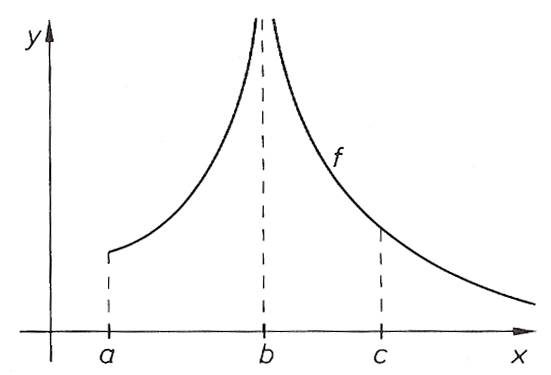
\includegraphics[width=4.5cm]{./bilder/unbeschraenkteFunktion.png}\\
    unbeschr\"ankte Funktion
  \end{multicols}
  
  
    
    
\subsubsection{Prinzip der Restfl\"ache}
  Wenn $\lim\limits_{t \rightarrow \infty} \int\limits^{\infty}_{t} f(x) dx = 0$, dann konvergiert
  $\int\limits_a^{\infty} f(x) dx$ und umgekehrt.

\subsubsection{Majorantenprinzip (konvergent)}
  Um nachzuweisen, ob eine Funktion $|f(x)| \geq 0$ konvergiert, wird eine zweite
  Funktion $g(x) \geq |f(x)|$ (Majorante) gesucht. Konvergiert $\int\limits_a^{\infty} g(x) dx$,
  dann konvergiert auch $\int\limits_a^{\infty} f(x) dx$. ($x \in [a, \infty)$)

\subsubsection{Minorantenprinzip (divergent)}
  Um nachzuweisen, ob eine Funktion $f(x)$ divergiert, wird eine zweite
  Funktion $0 \leq g(x) \leq f(x)$ (Minorante) gesucht. Divergiert
  $\int\limits_a^{\infty} g(x) dx$,
  dann divergiert auch $\int\limits_a^{\infty} f(x) dx$. ($x \in [a, \infty)$)
  